\documentclass[a4paper,12pt]{scrreprt}

%\usepackage[utf8]{inputenc}
\usepackage[ngerman]{babel}
\usepackage[T1]{fontenc}

\usepackage{setspace}
\usepackage{geometry}
\usepackage{graphicx}
\usepackage{amsmath}
\usepackage{csquotes}
%usepackage[backend=biber,style=numeric]{biblatex}
\usepackage[backend=biber]{biblatex}
\addbibresource{literatur.bib}
\usepackage{lastpage}
\usepackage{hyperref}

\geometry{
	left = 3cm,
	right = 2.5cm,
	top = 2.5cm,
	bottom = 2.5cm
}

\usepackage{fancyhdr}
\pagestyle{fancy}

\fancyhf{} % alles löschen

% Kopfzeile
\fancyhead[L]{\rightmark}
\fancyhead[C]{IRIS}
\fancyhead[R]{
\includegraphics[width=0.8cm]{images/BulmeLogo.png}}
\renewcommand{\headrulewidth}{0.4pt}
% Fußzeile
\fancyfoot[L]{Kalcher Linda\\ Tartler Katrin} 
\fancyfoot[C]{Diplomarbeit\\ 2025/26, 5AHEL}
\fancyfoot[R]{Seite \thepage \ von \pageref{LastPage}}
\renewcommand{\footrulewidth}{0.4pt}

\fancypagestyle{plain}{
\fancyhf{}
% Kopfzeile
\fancyhead[L]{\leftmark}
\fancyhead[C]{IRIS}
\fancyhead[R]{
\includegraphics[width=0.8cm]{images/BulmeLogo.png}}
\renewcommand{\headrulewidth}{0.4pt}
% Fußzeile
\fancyfoot[L]{Kalcher Linda\\ Tartler Katrin} 
\fancyfoot[C]{Diplomarbeit\\ 2025/26, 5AHEL}
\fancyfoot[R]{Seite \thepage \ von \pageref{LastPage}}
\renewcommand{\footrulewidth}{0.4pt}
}

\begin{document}

\begin{titlepage}
\centering
% Oberer Bereich
\begin{minipage}{0.6\textwidth}
	\centering
	\large
	\textbf{HTBLuVA Graz-Gösting}\\
	Ibererstraße 15-21\\
	8051 Graz
\end{minipage}
\hfill
\begin{minipage}{0.35\textwidth}
	\centering
	
\includegraphics[width=4cm]{images/BulmeLogo.png}
\end{minipage}

\vspace{3cm}

% Abteilung
{\LARGE Abteilung für}\\[0.3cm]
{\LARGE Elektronik und Technische Informatik}

\vspace{3cm}

% Diplomarbeit
{\Huge \textbf{DIPLOMARBEIT}}\\[1.2cm]

{\LARGE IRIS - Infant Recognition and Intelligence System}

\vfill

% Unterer Bereich (TOP-AUSRICHTUNG!)
% Unterer Bereich
\begin{minipage}[t]{0.55\textwidth}
\textbf{Ausgeführt im Schuljahr 2025/26 von:}\\[0.1cm]

Linda Kalcher [K]  \hspace{1cm} 5AHEL \\
Katrin Tartler [T] \hspace{1cm} 5AHEL
\end{minipage}
\hfill
\begin{minipage}[t]{0.4\textwidth}
\textbf{Betreut von:}\\[0.1cm]

Prof. DI DI Michelitsch Stephan, BEd, Bsc
\end{minipage}
\vspace{2cm}

Vorgelegt am 20. Mai 2026

\end{titlepage}
\newpage

\chapter*{Kurzbeschreibung}
\markboth{Kurzbeschreibung}{}

Mithilfe unseres Systems soll es Eltern ermöglicht werden, einen umfassenden und kontinuierlichen Überblick über ausgewählte Vitalwerte ihres Kindes zu erhalten.
Zu diesem Zweck wurde ein Reisebabybett mit verschiedenen Sensoren ausgestattet, die sowohl Bewegungen, Geräusche und Temperatur des Kindes erfassen können.
Die gewonnenen Daten werden in Echtzeit verarbeitet und visualisert. Die aufbereiteten Informationen 
sind online über eine Webanwendung (Progressive Web App, PWA) einsehbar.
\par\vspace{1em}
\noindent
Der Grundgedanke der Diplomarbeit war es, einen Beitrag zur Untersuchung des plötzlichen Kindstods zu leisten.
In erweiterter Form soll unser Datenerfassungssystem eine Grundlage schaffen, um neue Erkenntnisse in diesem Bereich zu ermöglichen und die Forschund zu unterstützen. 
\par\vspace{1em}
\noindent
Zur Überprüfung der Funktionsfähigkeit des Systems wurde ein spezieller Testroboter entwickelt, der typische Verhaltensweisen eines Babys simulieren kann.
Hierfür wurde eine handelsübliche Puppe technisch modifiziert und mit beweglichen Gliedmaßen ausgestattet. Zusätzlich kann der Roboter verschiedene Geräusche wiedergeben sowie eine Wärmesignatur erzeugen,
um realistische Bedingungen zu schaffen.
Auf diese Weise lassen sich die Sensoren und Auswertungsalgorithmen unter kontrollierten Bedingungen testen und optimieren.
\newpage

\chapter*{Abstract}
\markboth{Abstract}{}

With the help of our system, parents are enabled to obtain a comprehensive and continuous overview of selected vital parameters of their child.
For this purpose, a travel baby crib was equipped with various sensors capable of detecting the child’s movements, sounds, and temperature.
The collected data is processed and visualized in real time. The prepared information can be accessed online via a web application (Progressive Web App, PWA).
\par\vspace{1em}
\noindent
The core idea of this diploma thesis was to contribute to the study of sudden infant death syndrome (SIDS).
In an extended form, our data acquisition system is intended to provide a foundation for gaining new insights in this field and to support ongoing research efforts.
\par\vspace{1em}
\noindent
To verify the functionality of the system, a dedicated test robot was developed that can simulate typical infant behavior.
For this purpose, a commercially available doll was technically modified and equipped with movable limbs. In addition, the robot is capable of reproducing various sounds and generating a thermal signature in order to create realistic conditions.
This approach allows the sensors and data processing algorithms to be tested and optimized under controlled conditions.
\newpage
\chapter*{Eidesstattliche Erklärung}
\markboth{Eidesstattliche Erklärung}{}

Hiermit versichere ich, dass ich die vorliegende Arbeit selbstständig verfasst und keine anderen Hilfsmittel als die angegebenen benutzt habe.
Die Stellen, die anderen Werken (Büchern , Videos, Dokumenten, WebSites, usw.) wörtlich oder sinngemäß entnommen sind, habe ich unter Angabe der Quelle und Einhaltung der Regeln wissenschaftlichen Zitierens kenntlich gemacht.
Diese Versicherung umfasst auch in der Arbeit verwendete bildliche Darstellungen, Tabellen, Skizzen und Zeichnungen. Für die Erstellung der Arbeit habe ich auch folgende Hilfsmittel generativer KI-Tools ChatGPT und Copilot 
zu folgendem Zweck verwendet: Recherche, Quellenangabe und Formulierungshilfe.
Die verwendeten Hilfsmittel wurden vollständig und wahrheitsgetreu inkl. Produktversion und Prompt ausgewiesen.\\\\
\\\\

\noindent
\begin{minipage}[t]{0.45\textwidth}
\rule{\textwidth}{0.4pt}\\
Datum, Ort
\end{minipage}
\hfill
\begin{minipage}[t]{0.45\textwidth}
\rule{\textwidth}{0.4pt}\\
Unterschrift
\end{minipage}
\\\\
\\\\
\\\\
\begin{minipage}[t]{0.45\textwidth}
\rule{\textwidth}{0.4pt}\\
Datum, Ort
\end{minipage}
\hfill
\begin{minipage}[t]{0.45\textwidth}
\rule{\textwidth}{0.4pt}\\
Unterschrift
\end{minipage}

\newpage

\chapter*{Danksagung}
\markboth{Danksagung}{}
Wir bedanken und bei unserem Betreuer Herrn Professor DI DI Stephan Michelitsch, BEd, Bsc, welcher 
uns von Themenfindung bis zum Schreiben der vorliegenden Diplomarbeit durchwegs unterstützt hat.

\noindent
Wir bedanken uns bei Fachleher Ing. Niki Schellnegger für die Hilfe beim Ätzen unserer Platinen.

\noindent
Außerdem wollen wir uns bei unsereren Familien für die Untertützung beim Korrekturlesen, dem Bereitstellen 
von Werkzeug und der Anschaffung von Materialien bedanken.  


\newpage



\chapter{Theorie}
\section{Wie kam es dazu?}

\section{Plötzlicher Kindstod Theorie}
Unter dem Begriff Plötzlicher Kindstod versteht man das Versterben eines Babys welches
das erste Lebensjahr noch nicht vollendet hat und unter keinerlei Vorerkrankungen litt.
Im Zuge der Diagnose muss auch der Fundort des leblosen Kindes untersucht werden um einen Unfalltod, 
durch Ersticken an einer Decke, Kuscheltiers, etc. auszuschließen. 
Deshalb handelt es sich hierbei auch um eine Ausschlussdiagnose. 
In Österreich und anderen Industrienationen der Welt ist SIDS eine der häufigsten diagnostizierten Todesursachen.\cite{meinmed_sids}
Zudem belegen Statistiken, dass der Plötzliche Kindstod vor allem in den Wintermonaten auftritt und meist im Schlaf. \cite{der-ploetzliche-saeuglingstod-epidemiologie-aetiologie-pathophysiologie-und-differenzialdiagnostik} \cite{Poets2020}

\section{Theorie zum allgemeineren System}
%Was kann man zum auslesen von Vitalwerten bzw. unseren Aufnahmedaten so an theorie finden?
%muss nicht wirklich schon genau auf unser System bezogen sein

\section{Was gibt es schon?}
\subsection{Markt}
%KI gesteuerte Babyphone usw.

\subsection{Forschung}
%Babysprachentheorie
%med uni graz Ki Modell

%Bettchen Theorie 

%Roboter Theorie 
\section{Testroboter}
\subsection{BLE und Interface}
\subsubsection{BLE Architektur} 
Bluetooth Low Energy ist eine Bluetooth Protokoll, das im Vergleich zu Classic Bluetooth einen geringeren Stromverbrauch hat und somit auch einen niedrigere Datentransferrate erreicht.
Es wird vor allem im Bereich Internet of Things (IoT) und für Kommunikation mit Messsensoren benutzt.
BLE ist nicht kompatibel mit Classic Bluetooth. 
Das BLE Protokoll ist in drei Schichten geteilt.
\begin{itemize}
\item Application Layer
\item Host Layer
\item und Controller Layer
\item \end{itemize}
siehe Abbildung \ref{fig:ble_architektur}

\begin{figure}[htbp]
\centering
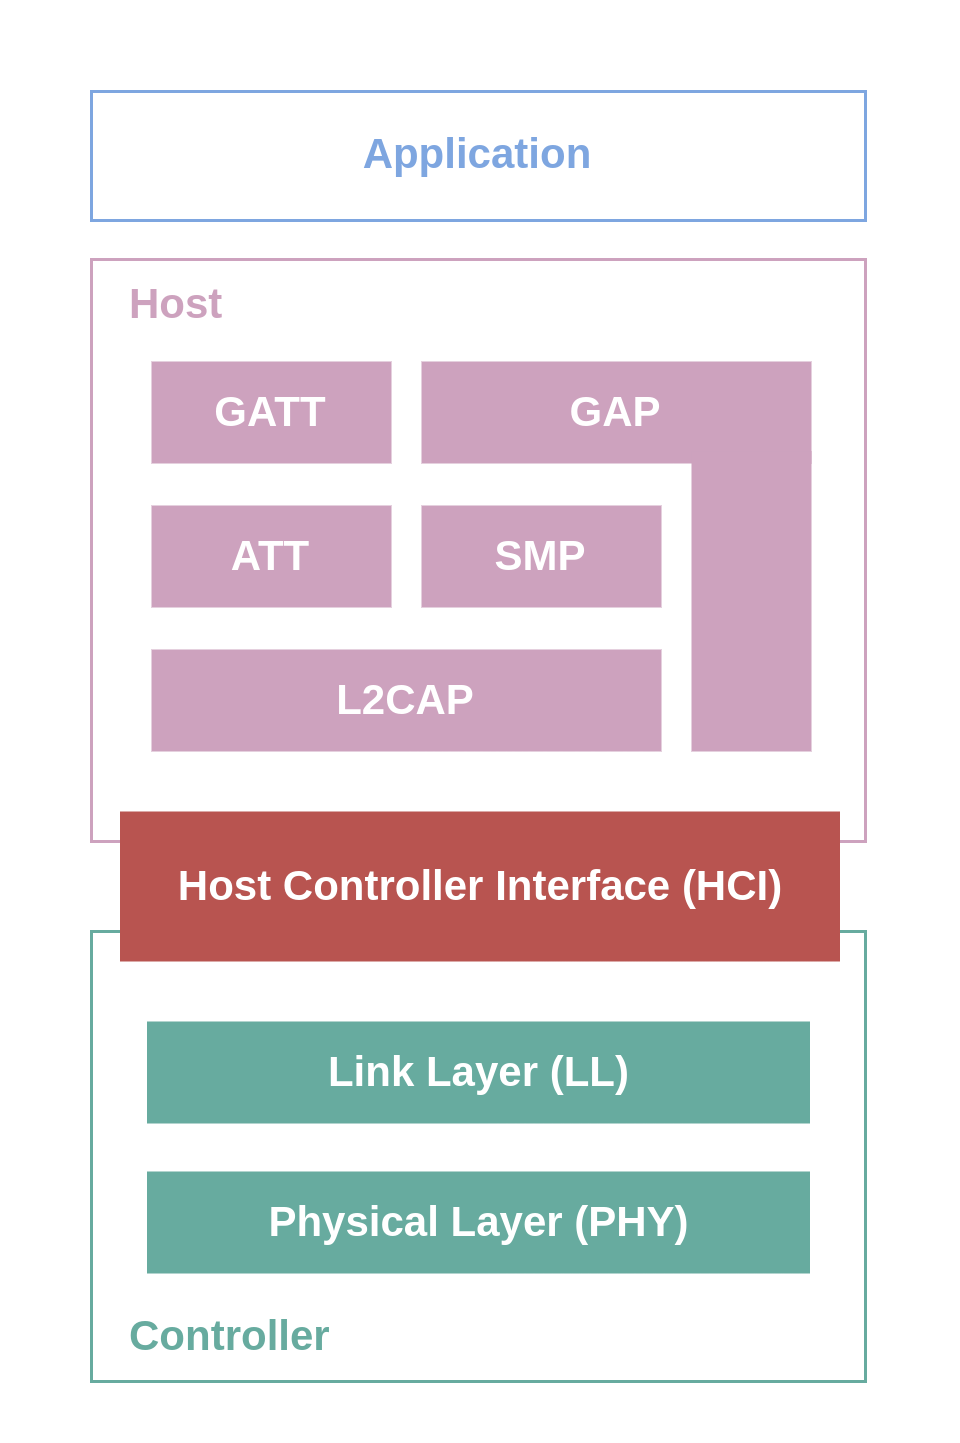
\includegraphics[width=7cm]{images/ble-architecture.png}
\caption{BLE Architektur}
\label{fig:ble_architektur}
\end{figure}

\noindent
In der Application Layer können wir unsere Anwendung mit BLE realisieren. Hier implementiert man seine Anforderungen.In der Host Layer findet die Kommunikation zwischen Benutzeranwendung und Controllinterface der Hardware statt, man nennt diese Ebene auch Host Stack. Der in Kombination mit dem Controller Stack den Bluetooth Stack bildet. Alle relevanten Bluetooth LE Protokolle der Hostseite sind hier implementiert.\cite{espressif_bluetooth_architecture} In der letzten Schicht, der Controller Layer finden die physical und die link Layer ihren Platz. Sie interagieren direkt mit der Hardware. Die BLE-Protokolle der Host Schicht sind GAP, ATT, GATT, SMP und L2CAP.\cite{espressif_ble_intro}
\newpage

\subsubsection{GAP (Generic Accsess Profile)}
Ist für die Verbindung von zwei BLE-Geräten verantwortlich. Das Protokoll ist in 3 verschiedene Modi geteilt je nachdem welcher Verbindungsgrad erfüllt ist. Innerhalb dieser gibt es Rollen die den Geräten zugeteilt sind. 
 
\begin{figure}[h]
\centering
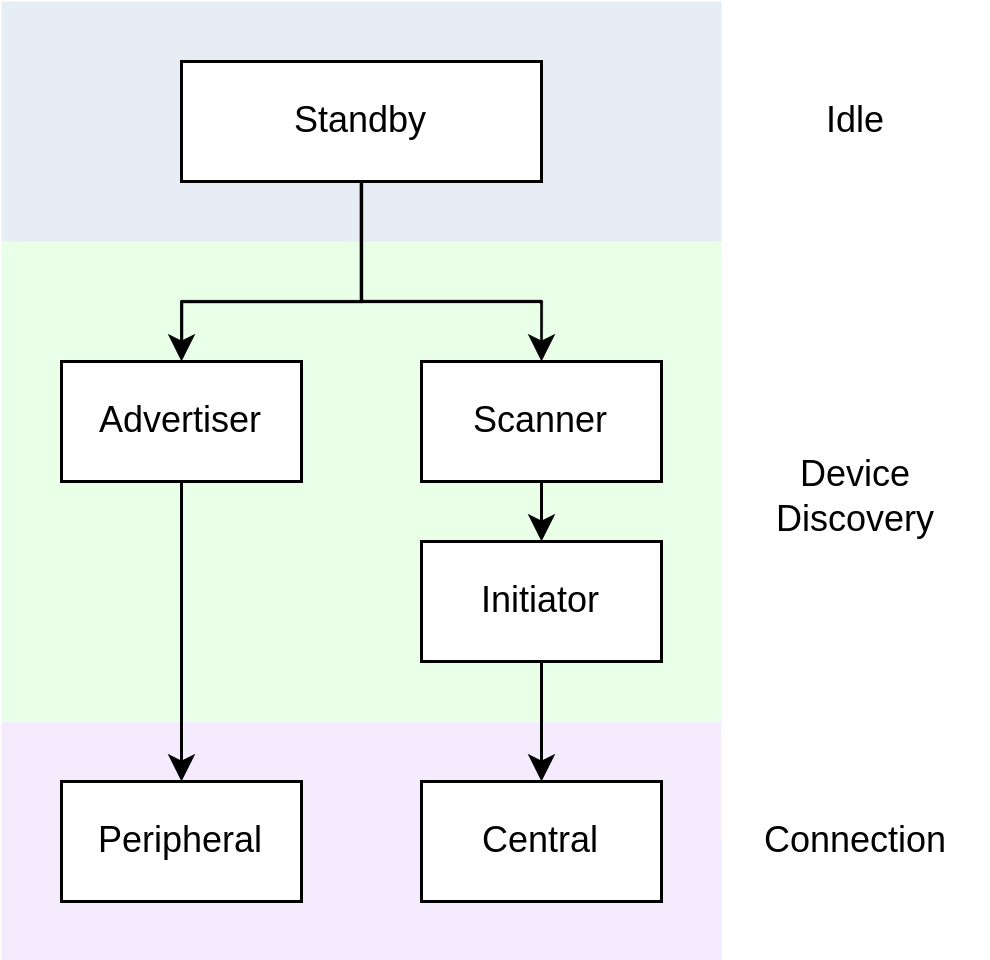
\includegraphics[width = 4cm]{images/ble-gap.png}
\caption{BLE GAP}
\label{fig:ble_gap}
\end{figure}
\noindent
In unserem Projekt übernimmt der ESP32 die Rolle des Servers, und der Laptop ist der Client. 
Im GAP werden diese Rollen mit Peripheral (Server) und Central (Client) bezeichnet. \cite{espressif_ble_intro} Anhand von Abbildung \ref{fig:ble_gap_bsp} lässt sich der Verbindungsaufbau und die unterschiedlichen Rollen welche die Teilnehmener dabei annehmen nachvollziehen.
\begin{figure}[h]
\centering
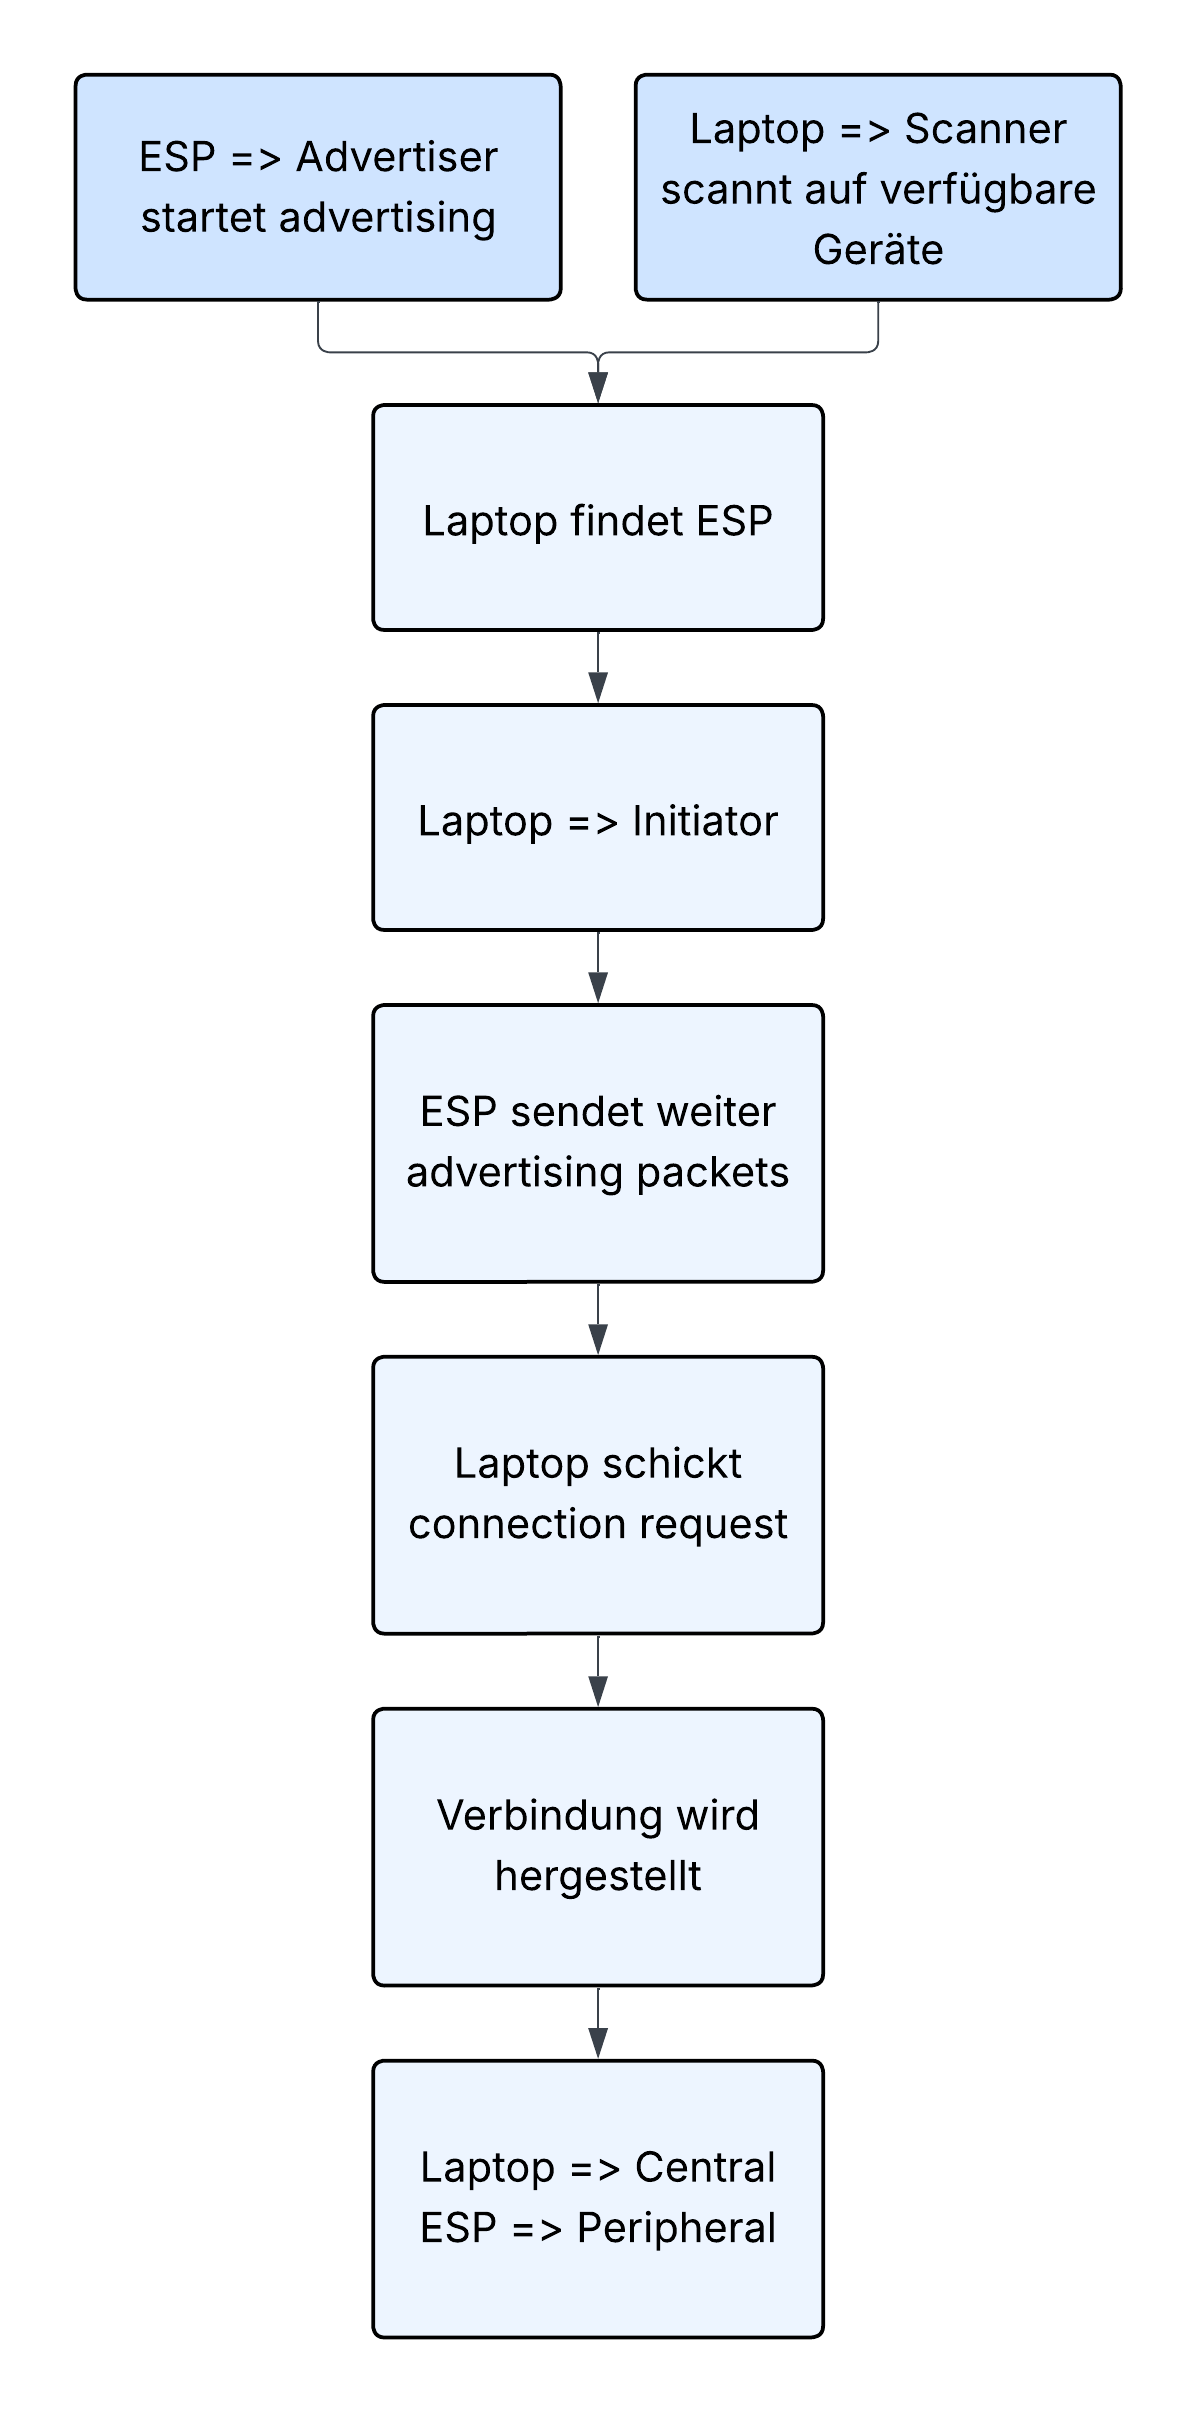
\includegraphics[width = 6cm]{images/ble-gap_bsp.png}
\caption{GAP Verbindungsaufbau}
\label{fig:ble_gap_bsp}
\end{figure}


\subsubsection{GATT (Generic Attribute Profile)}
Dieses Protokoll basiert auf einer hierarchischen Einteilung von Characteristic, Service und Profile. Hier legt der Benutzter eine Anwendung anhand der vorgegebenen Struktur von BLE an. Diese wird in der ATT Layer technisch umgesetzt und gespeichert. siehe \ref{ATT}.

\noindent
Characteristics sind Datenstrukturen die mit Attributen aufgebaut sind. Sie müssen ein Characteristic Declaration Attribute und ein Characteristic Value Attribute beinhalten. Optional gibt es die Möglichkeit noch weitere Descriptor Attributes in einer Characteristic zu implementieren.

\noindent
Services sind ebenfalls mit Attributen aufgebaut. Ein sogennates Service Declaration Attribute muss definiert sein. In einem Service sind mehrere Characteristics mit einer ähnlichen Funktion oder zusammenhängenden Funktionen gesammelt.

\noindent
Profiles sind die übergeordnetesten Instanzen. Sie müssen gewisse Services haben muss um einen Standard zu erfüllen. Bei der Verwendung von BLE werden sie im Programmcode nicht definiert, wie Characteristics und Services. Ein Profile entsteht in dieser Hinsicht in einem Projekt nur konzeptionell. \cite{espressif_ble_intro}



\subsubsection{ATT (Attribute Protocol)} \label{ATT}
Auf dieser Ebene passiert die technische Umsetzung des GATT. Eine dort erzeugt Charakteristik wird am Server Device als Attribute gespeichert. Attribute sind strukturiert in Type, Value und Permission. Dabei werden sie im Speicher meist als Arrays angelegt- Attribute Table. Der Type eines Attributs ist ein 32- oder öfter benutzte 128bit langer UUID (Universally Unique IDentifier). \cite{espressif_ble_intro}

\subsubsection{L2CAP (Logic Link Control and Adaption Layer Protocol)}
L2CAP ist für die Datenpaketverwaltung zuständig. Es wird auf Client- sowie auf Hostseite benutzt. Zu den Aufgaben gehören unter anderem Multiplexing, Segementierung und Wiederzusammensetzung der Daten. \cite{ti_ble_l2cap}

\subsubsection{SMP (Security Manager Protocol )}
Ist das Sicherheitsprotokoll von BLE, es ist ein Untermodul von GAP. \cite{espressif_bluetooth_security}



%\subsection{JLC ?}

\subsection{Realtime System}

\subsection{Bewegungssimulation}
%Motortheorie
%Vergleich Stepper vs. Servo

\subsection{Geräuschsimulation}
%Modul erklären
%Lautsprecher Theorie

\subsection{Wärmesimulation}
\subsubsection{Keramikwiderstände}


%PT100 Regelung? das was mc geyappt hat
%Keramikwiderstände vs. Heizelemente



\section{Platinendesign}
\subsection{KiCad}
%3d model



\section{3D Druck}







\end{document}

